\documentclass[mathserif]{beamer}

\setbeamertemplate{frametitle}[default][center]%Centers the frame title.
\setbeamertemplate{navigation symbols}{}%Removes navigation symbols.
\setbeamertemplate{footline}{\raisebox{5pt}{\makebox[\paperwidth]{\hfill\makebox[10pt]{\scriptsize\insertframenumber}}}}
\setbeamertemplate{caption}[numbered]

%\newcommand{\tth}   {\mbox{$\theta$}}
\newcommand{\thh}   {\mbox{$\theta$}}
\newcommand{\su}   {\mbox{$\sigma^2$}}
\newcommand{\so}   {\mbox{$\sigma_0^2$}}
\newcommand{\ko}   {\mbox{$\kappa_0$}}
\newcommand{\no}   {\mbox{$\nu_0$}}
\newcommand{\mo}   {\mbox{$\mu_0$}}
\newcommand{\ti}   {\mbox{$\tilde{x}$}}
\newcommand{\la}   {\mbox{$\lambda$}}
\newcommand{\bx}   {\mbox{$\bm{x}$}}
\newcommand{\bZ}   {\mbox{$\bm{Z}$}}
\newcommand{\bX}   {\mbox{$\bm{X}$}}
\newcommand{\bY}   {\mbox{$\bm{Y}$}}
\newcommand{\bA}   {\mbox{$\bm{A}$}}
\newcommand{\ba}   {\mbox{$\bm{a}$}}
\newcommand{\bb}   {\mbox{$\bm{b}$}}
\newcommand{\bt}   {\mbox{$\bm{t}$}}
\newcommand{\bz}   {\mbox{$\bm{z}$}}
\newcommand{\bw}   {\mbox{$\bm{w}$}}
\newcommand{\bbeta}   {\mbox{$\bm{\beta}$}}

\newcommand{\be}   {\mbox{$\bm{e}$}}
\newcommand{\bu}   {\mbox{$\bm{u}$}}
\newcommand{\bv}   {\mbox{$\bm{v}$}}
\newcommand{\sig}   {\mbox{$\Sigma$}}
\newcommand{\sigx}   {\mbox{$\Sigma_{XX}$}}
\newcommand{\sigxy}   {\mbox{$\Sigma_{XY}$}}
\newcommand{\tr}   {\mbox{$\text{tr}$}}
\newcommand{\ddet}   {\mbox{$\text{det}$}}
\newcommand\independent{\protect\mathpalette{\protect\independenT}{\perp}}
\def\independenT#1#2{\mathrel{\rlap{$#1#2$}\mkern2mu{#1#2}}}

\newcommand{\Expect}[1]{\ensuremath{\mathbf{E}\left[ #1 \right]}}
%\newcommand{\Var}[1]{\ensuremath{\mathrm{Var}\left[ #1 \right]}}
%\newcommand{\Cov}[1]{\ensuremath{\mathrm{Cov}\left[ #1 \right]}}
\newcommand{\MSE}{\ensuremath{\mathrm{MSE}}}
\newcommand{\RSS}{\ensuremath{\mathrm{RSS}}}
\newcommand{\Prob}[1]{\ensuremath{\mathrm{Pr}\left( #1 \right)}}
\newcommand{\ProbEst}[1]{\ensuremath{\widehat{\mathrm{Pr}}\left( #1 \right)}}
\DeclareMathOperator*{\argmin}{argmin} % thanks, wikipedia!
\DeclareMathOperator*{\argmax}{argmax} % thanks, wikipedia!
\DeclareMathOperator*{\sgn}{sgn} % thanks, wikipedia!

\newcommand{\lam}{\lambda}
\newcommand{\bmu}{\bm{\mu}}
%\newcommand{\bx}{\ensuremath{\mathbf{X}}}
\newcommand{\X}{\ensuremath{\mathbf{X}}}
\newcommand{\w}{\ensuremath{\mathbf{w}}}
\newcommand{\h}{\ensuremath{\mathbf{h}}}
\newcommand{\V}{\ensuremath{\mathbf{V}}}
%\newcommand{\tr}{\operatorname{tr}}

%\newcommand{\bx}{\ensuremath{\mathbf{X}}}
%\newcommand{\X}{\ensuremath{\mathbf{x}}}
%\newcommand{\w}{\ensuremath{\mathbf{w}}}
%\newcommand{\h}{\ensuremath{\mathbf{h}}}
%\newcommand{\V}{\ensuremath{\mathbf{v}}}
%\newcommand{\Cov}{\text{Cov}}
%\newcommand{\Var}{\text{Var}}

\DeclareMathOperator{\var}{Var}
\DeclareMathOperator{\cov}{Cov}
\newcommand{\Var}[1]{\ensuremath{\mathrm{Var}\left[ #1 \right]}}
\newcommand{\Cov}[1]{\ensuremath{\mathrm{Cov}\left[ #1 \right]}}


\newcommand{\indep}{\rotatebox{90}{\ensuremath{\models}}}
\newcommand{\notindep}{\not\hspace{-.05in}\indep}







\usepackage{float,amsmath,bm}
\usepackage{amssymb}
\usepackage{epsfig}
\usepackage{graphicx}
\usepackage{fancyhdr}
\usepackage{multirow}
\floatstyle{boxed}
\newfloat{code}{tp}{code}
\floatname{code}{Code Example}
\newcommand{\tth}   {\mbox{$\theta$}}
\newcommand{\thh}   {\mbox{$\theta$}}
\newcommand{\su}   {\mbox{$\sigma^2$}}
\newcommand{\so}   {\mbox{$\sigma_0^2$}}
\newcommand{\ko}   {\mbox{$\kappa_0$}}
\newcommand{\no}   {\mbox{$\nu_0$}}
\newcommand{\mo}   {\mbox{$\mu_0$}}
\newcommand{\ti}   {\mbox{$\tilde{x}$}}
\newcommand{\la}   {\mbox{$\lambda$}}
\newcommand{\bx}   {\mbox{$\bm{x}$}}
\newcommand{\bZ}   {\mbox{$\bm{Z}$}}
\newcommand{\bX}   {\mbox{$\bm{X}$}}
\newcommand{\bY}   {\mbox{$\bm{Y}$}}
\newcommand{\bA}   {\mbox{$\bm{A}$}}
\newcommand{\ba}   {\mbox{$\bm{a}$}}
\newcommand{\bb}   {\mbox{$\bm{b}$}}
\newcommand{\bt}   {\mbox{$\bm{t}$}}
\newcommand{\bz}   {\mbox{$\bm{z}$}}
\newcommand{\bw}   {\mbox{$\bm{w}$}}
\newcommand{\bbeta}   {\mbox{$\bm{\beta}$}}

\newcommand{\be}   {\mbox{$\bm{e}$}}
\newcommand{\bu}   {\mbox{$\bm{u}$}}
\newcommand{\bv}   {\mbox{$\bm{v}$}}
\newcommand{\sig}   {\mbox{$\Sigma$}}
\newcommand{\sigx}   {\mbox{$\Sigma_{XX}$}}
\newcommand{\sigxy}   {\mbox{$\Sigma_{XY}$}}
\newcommand{\tr}   {\mbox{$\text{tr}$}}
\newcommand{\ddet}   {\mbox{$\text{det}$}}
\newcommand\independent{\protect\mathpalette{\protect\independenT}{\perp}}
\def\independenT#1#2{\mathrel{\rlap{$#1#2$}\mkern2mu{#1#2}}}

\newcommand{\Expect}[1]{\ensuremath{\mathbf{E}\left[ #1 \right]}}
%\newcommand{\Var}[1]{\ensuremath{\mathrm{Var}\left[ #1 \right]}}
%\newcommand{\Cov}[1]{\ensuremath{\mathrm{Cov}\left[ #1 \right]}}
\newcommand{\MSE}{\ensuremath{\mathrm{MSE}}}
\newcommand{\RSS}{\ensuremath{\mathrm{RSS}}}
\newcommand{\Prob}[1]{\ensuremath{\mathrm{Pr}\left( #1 \right)}}
\newcommand{\ProbEst}[1]{\ensuremath{\widehat{\mathrm{Pr}}\left( #1 \right)}}
\DeclareMathOperator*{\argmin}{argmin} % thanks, wikipedia!
\DeclareMathOperator*{\argmax}{argmax} % thanks, wikipedia!
\DeclareMathOperator*{\sgn}{sgn} % thanks, wikipedia!

\newcommand{\lam}{\lambda}
\newcommand{\bmu}{\bm{\mu}}
%\newcommand{\bx}{\ensuremath{\mathbf{X}}}
\newcommand{\X}{\ensuremath{\mathbf{X}}}
\newcommand{\w}{\ensuremath{\mathbf{w}}}
\newcommand{\h}{\ensuremath{\mathbf{h}}}
\newcommand{\V}{\ensuremath{\mathbf{V}}}
%\newcommand{\tr}{\operatorname{tr}}

%\newcommand{\bx}{\ensuremath{\mathbf{X}}}
%\newcommand{\X}{\ensuremath{\mathbf{x}}}
%\newcommand{\w}{\ensuremath{\mathbf{w}}}
%\newcommand{\h}{\ensuremath{\mathbf{h}}}
%\newcommand{\V}{\ensuremath{\mathbf{v}}}
%\newcommand{\Cov}{\text{Cov}}
%\newcommand{\Var}{\text{Var}}

\DeclareMathOperator{\var}{Var}
\DeclareMathOperator{\cov}{Cov}
\newcommand{\Var}[1]{\ensuremath{\mathrm{Var}\left[ #1 \right]}}
\newcommand{\Cov}[1]{\ensuremath{\mathrm{Cov}\left[ #1 \right]}}


\newcommand{\indep}{\rotatebox{90}{\ensuremath{\models}}}
\newcommand{\notindep}{\not\hspace{-.05in}\indep}






%\usepackage{fontspec}
%\setmainfont{Tahoma}

%\newcommand{\lam}{\lambda}
%\newcommand{\bmu}{\bm{\mu}}
%%\newcommand{\bx}{\ensuremath{\mathbf{X}}}
%\newcommand{\X}{\ensuremath{\mathbf{x}}}
%\newcommand{\w}{\ensuremath{\mathbf{w}}}
%\newcommand{\h}{\ensuremath{\mathbf{h}}}
%\newcommand{\V}{\ensuremath{\mathbf{v}}}
%\newcommand{\cov}{\text{Cov}}
%\newcommand{\var{\text{Var}}}

%\DeclareMathOperator{\var}{Var}
%\DeclareMathOperator{\cov}{Cov}

%\newcommand{\indep}{\rotatebox{90}{\ensuremath{\models}}}
%\newcommand{\notindep}{\not\hspace{-.05in}\indep}

\usepackage{graphicx} %The mode "LaTeX => PDF" allows the following formats: .jpg  .png  .pdf  .mps
\graphicspath{{./PresentationPictures/}} %Where the figures folder is located
\usepackage{listings}
\usepackage{media9}
\usepackage{movie15}
\addmediapath{./Movies/}

\newcommand{\beginbackup}{
   \newcounter{framenumbervorappendix}
   \setcounter{framenumbervorappendix}{\value{framenumber}}
}
\newcommand{\backupend}{
   \addtocounter{framenumbervorappendix}{-\value{framenumber}}
   \addtocounter{framenumber}{\value{framenumbervorappendix}} 
}


%\usepackage{algorithm2e}
\usepackage[ruled,lined]{algorithm2e}
\def\algorithmautorefname{Algorithm}
\SetKwIF{If}{ElseIf}{Else}{if}{then}{else if}{else}{endif}
%\usepackage{times}
%\usepackage[tbtags]{amsmath}
%\usepackage{amssymb}
\usepackage{amsfonts}
%\usepackage{slfortheorems}
\usepackage{epsfig}
\usepackage{graphicx}
\usepackage[small]{caption}
%\usepackage[square]{natbib}
%\newcommand{\newblock}{}
%\bibpunct{(}{)}{;}{a}{}{,}
%\bibliographystyle{ims}
%\usepackage[letterpaper]{geometry}
\usepackage{color}
\setlength{\parindent}{0pt}

\usepackage{natbib}
\bibpunct{(}{)}{;}{a}{}{,}
%\usepackage{hyperref}



%\usepackage{zref-savepos}
%
%\newcounter{restofframe}
%\newsavebox{\restofframebox}
%\newlength{\mylowermargin}
%\setlength{\mylowermargin}{2pt}
%
%\newenvironment{restofframe}{%
%    \par%\centering
%    \stepcounter{restofframe}%
%    \zsavepos{restofframe-\arabic{restofframe}-begin}%
%    \begin{lrbox}{\restofframebox}%
%}{%
%    \end{lrbox}%
%    \setkeys{Gin}{keepaspectratio}%
%    \raisebox{\dimexpr-\height+\ht\strutbox\relax}[0pt][0pt]{%
%    \resizebox*{!}{\dimexpr\zposy{restofframe-\arabic{restofframe}-begin}sp-\zposy{restofframe-\arabic{restofframe}-end}sp-\mylowermargin\relax}%
%        {\usebox{\restofframebox}}%
%    }%
%    \vskip0pt plus 1filll\relax
%    \mbox{\zsavepos{restofframe-\arabic{restofframe}-end}}%
%    \par
%}


\usepackage{tikz}
\usetikzlibrary{arrows}

%\usepackage[usenames,dvipsnames]{xcolor}
\usepackage{tkz-berge}
\usetikzlibrary{fit,shapes}

\usepackage{calc}
%%
%% The tikz package is used for doing the actual drawing.
%\usepackage{tikz}
%%
%% In order to be able to put arrowheads in the middle of directed edges, we need an extra library.
\usetikzlibrary{decorations.markings}
%%
%% The next line says how the "vertex" style of nodes should look: drawn as small circles.
\tikzstyle{vertex}=[circle, draw, inner sep=0pt, minimum size=6pt]
%%
%% Next, we make a \vertex command as a shorthand in place of \node[vertex} to get that style.
\newcommand{\vertex}{\node[vertex]}
%%
%% Finally, we declare a "counter", which is what LaTeX calls an integer variable, for use in
%% the calculations of angles for evenly spacing vertices in circular arrangements.
\newcounter{Angle}

\newtheoremstyle{example}
{\topsep} % space above
{\topsep} % space below
{} % body font
{} % indent
{\bf} % head font
{:} % punctuation between head and body
{0.5em} % space after head
{} % manually specify head
%{\thmname{#1}\thmnumber{ #2}\thmnote{:#3}} % manually specify head

\theoremstyle{example}
\newtheorem{ex}{Example}[section]

\newtheoremstyle{definition}
{\topsep} % space above
{\topsep} % space below
{} % body font
{} % indent
{\sc} % head font
{:} % punctuation between head and body
{0.5em} % space after head
{} % manually specify head
%{\thmname{#1}\thmnumber{ #2}\thmnote{:#3}} % manually specify head

\theoremstyle{definition}
\newtheorem{defn}{Definition}[section]

\theoremstyle{rem}
\newtheorem{rem}{Remark}[section]

\newtheoremstyle{theorem}
{\topsep} % space above
{\topsep} % space below
{} % body font
{} % indent
{\sc} % head font
{:} % punctuation between head and body
{0.5em} % space after head
{} % manually specify head
%{\thmname{#1}\thmnumber{ #2}\thmnote{:#3}} % manually specify head

\theoremstyle{theorm}
\newtheorem{thm}{Theorem}[section]



%%%to add in new counter for slides in beamer

%\setbeamertemplate{footline}{
%  \leavevmode%
%  \hbox{%
%  \begin{beamercolorbox}[wd=.333333\paperwidth,ht=2.25ex,dp=1ex,center]{author in head/foot}%
%    \usebeamerfont{author in head/foot}\insertshortauthor~~(\insertshortinstitute)
%  \end{beamercolorbox}%
%  \begin{beamercolorbox}[wd=.333333\paperwidth,ht=2.25ex,dp=1ex,center]{title in head/foot}%
%    \usebeamerfont{title in head/foot}\insertshorttitle
%  \end{beamercolorbox}%
%  \begin{beamercolorbox}[wd=.333333\paperwidth,ht=2.25ex,dp=1ex,right]{date in head/foot}%
%    \usebeamerfont{date in head/foot}\insertshortdate{}\hspace*{2em}
%    \insertframenumber{} \hspace*{2ex} % hier hat's sich ge�ndert
%  \end{beamercolorbox}}%
%  \vskip0pt%
%}

\newcommand{\blue}   {\textcolor{blue}}
\newcommand{\loss}   {\mbox{$L(\theta,\delta(x))$}}
\newcommand{\del}   {\mbox{$\delta(x)$}}
\newcommand{\frisk}   {\mbox{$ R(\tth, \del) = E_{\tth}[\loss]$}}
\newcommand{\prisk}   {\mbox{$ \rho(\pi, \del) = \int_{\Theta} \loss \textcolor{blue}{\pi(\theta|x)}\; d\theta$}}
\newcommand{\that}   {\mbox{$\hat{\theta}$}}

%%%%%

\newcommand*\oldmacro{}
\let\oldmacro\insertshortauthor
\renewcommand*\insertshortauthor{
  \leftskip=.3cm
\insertframenumber\,/\,\inserttotalframenumber\hfill\oldmacro}




%\excludecomment{notbeamer}
%\includecomment{beamer}



\title{Intro to Decision Theory}
\author{Rebecca C. Steorts \\ Bayesian Methods and Modern Statistics: STA 360/601}
\date{Lecture 3}

\begin{document}

\maketitle

\frame{
\frametitle{Please be patient with the Windows machine....}

\begin{figure}[htbp]
\begin{center}
\includegraphics[width=\textwidth]{classRoomComputing}
\label{default}
\end{center}
\end{figure}

}

\frame{
\frametitle{Topics}
\begin{itemize}
\item Loss function
\item Risk
\item Posterior Risk
\item Bayes risk
\item Bayes estimator
\item Minimax estimators
\item An Example
\end{itemize}


}

\frame{
\frametitle{A Nice Relaxation}

\begin{enumerate}
\item Derivations on the homework, you can write it up and scan it. 
\item Any computational piece must be done in R/Markdown and be reproducible (this includes the writing here). 
\end{enumerate}
What about file submissions. If you choose to do it as homework 1, submit as before. 
\vskip 1em
If you choose to submit with handwritten, R/Markdown, then you will need:
\begin{enumerate}
\item A .pdf file with clearly written problems (note anything that we can't read, won't be graded). 
\item Any computational piece must be done in R/Markdown and be reproducible (this includes the writing here).
\item You must attach all .pdf, .tex, .Rmd files above that are needed to grade your homework. If you're unsure, come and ask in office hours. 
\end{enumerate}
Other stuff that comes up (come talk to me)....

}

\frame{
\frametitle{Motivating Example: Skiing Anyone?}


\begin{figure}[htbp]
\begin{center}
\includegraphics[width=0.8\textwidth]{skiingSwiss}
\label{default}
\end{center}
\end{figure}




}

\frame{
\frametitle{Motivating Example: Skiing Anyone?}


\begin{figure}[htbp]
\begin{center}
\includegraphics[width=0.8\textwidth]{skiing2}
\label{default}
\end{center}
\end{figure}




}

\frame{
\frametitle{Risk and Skiing}

\center
What types of things could go wrong?


}



\frame{
One way Bayesian methods are often used are in making optimal decisions.
\vskip 1em
In statistical decision theory, we formalize good and bad results with a loss function.
}

%\frame{
%\begin{itemize}
%\item A loss function 
%$\loss$
% is a function of unknown parameter $\theta \in \Theta$.
%\item  $\del$ is a decision based on the data
%$x \in X$.  
%\end{itemize}
%
%\begin{itemize}
%\item For example, $\del=n^{-1}\sum_{i=1}^n x_i$ might be the sample mean, and $\theta$ might be the true mean.  
%\item The loss function determines
%the penalty for deciding how well $\del$ estimates $\tth$.
%\end{itemize}
%One discrete loss (0-1):
%\begin{align*}
%\loss=\begin{cases}
%0 & \text{ if }\del=\theta,\\
%1 & \text{ if }\del\ne\theta,
%\end{cases}
%\end{align*}
%Another loss is squared error: $\loss = 
%(\tth - \del)^2.$\\
%\vskip 1em
%Why do we use such choices?
%
%
%
%}


\frame{
\frametitle{What is loss?}
\begin{itemize}
\item Loss function 
$\loss$
 is a function of unknown parameter $\theta \in \Theta$.
\item  $\del$ is a decision based on the data
$x \in X$.  
\end{itemize}

\vskip 1em

What are some examples of $\del$?

\begin{itemize}
\item Does Duke win or lose a given basketball game (0-1 loss). 
\item Two player game based on set of non-binary rules (point system).\footnote{(Discrete loss, for this example see Ch 5
 of Baby Bayes notes).}
\item Sample average of the data. 
\end{itemize}
Back to our skiing example: $\theta$: probability that you tear your ACL. $\delta$: estimator of $\theta.$
}

\frame{
\frametitle{Loss}
\begin{itemize}
%\item For example, $\del=n^{-1}\sum_{i=1}^n x_i$ might be the sample mean, and $\theta$ might be the true mean.  
\item The loss function determines
the penalty for deciding how well $\del$ estimates $\tth$.
\end{itemize}
One discrete loss (0-1):
\begin{align*}
\loss=\begin{cases}
0 & \text{ if }\del=\theta,\\
1 & \text{ if }\del\ne\theta,
\end{cases}
\end{align*}
Another loss is squared error: $\loss = $
%(\tth - \del)^2.$\\
\vskip 1em
Why do we use such choices?



}



\frame{
\frametitle{What is risk?}

We understand loss. But how do we understand a concept of ``risk" in a formal setting?
\vskip 1 em

Example: ``I hate getting wet in the rain. How can I minimize the risk that I will never get wet?"

\vskip 1 em

Intuition: Just always carry an umbrella. 

\vskip 1 em

We will come back to this example later. Now, some defintitions.


}




\frame{
\frametitle{Frequentist Risk (Risk)}

The \blue{frequentist risk} (risk) is
$$\frisk = \int_{X} L(\theta,\delta) \blue{f(x|\theta)} \; dx.$$
where $\tth$ is held fixed and the expectation is taken over $X.$

\vskip 1 em
Risk measures the long-term average loss resulting from using $\delta.$


}

\frame{
\begin{figure}[htdp]
\begin{center}
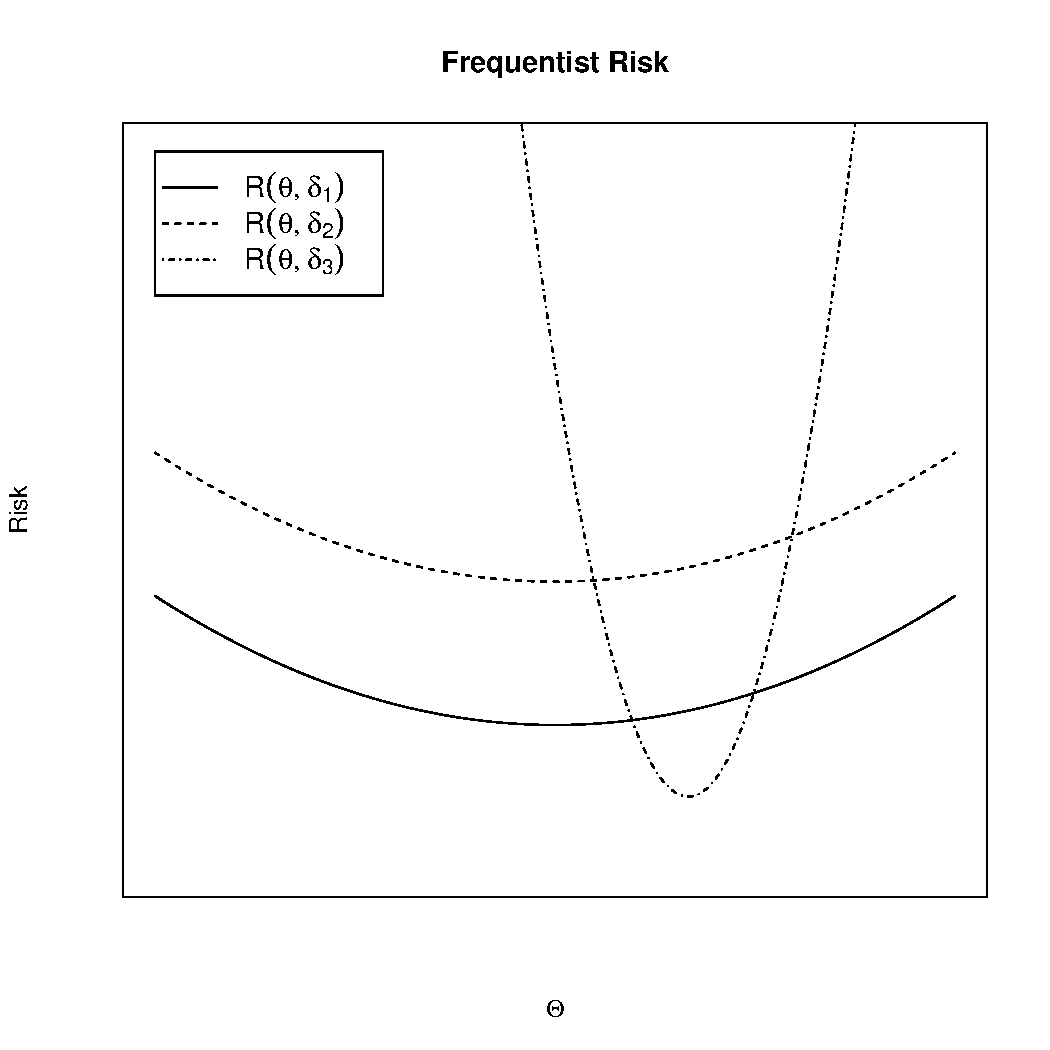
\includegraphics[width = .7\textwidth]{Lec2p1fig1.pdf}
\caption{Shows the risk of three different decisions as a function of $\theta \in \Theta$}
\label{default}
\end{center}
\end{figure}
}

\frame{
\begin{figure}[htdp]
\begin{center}
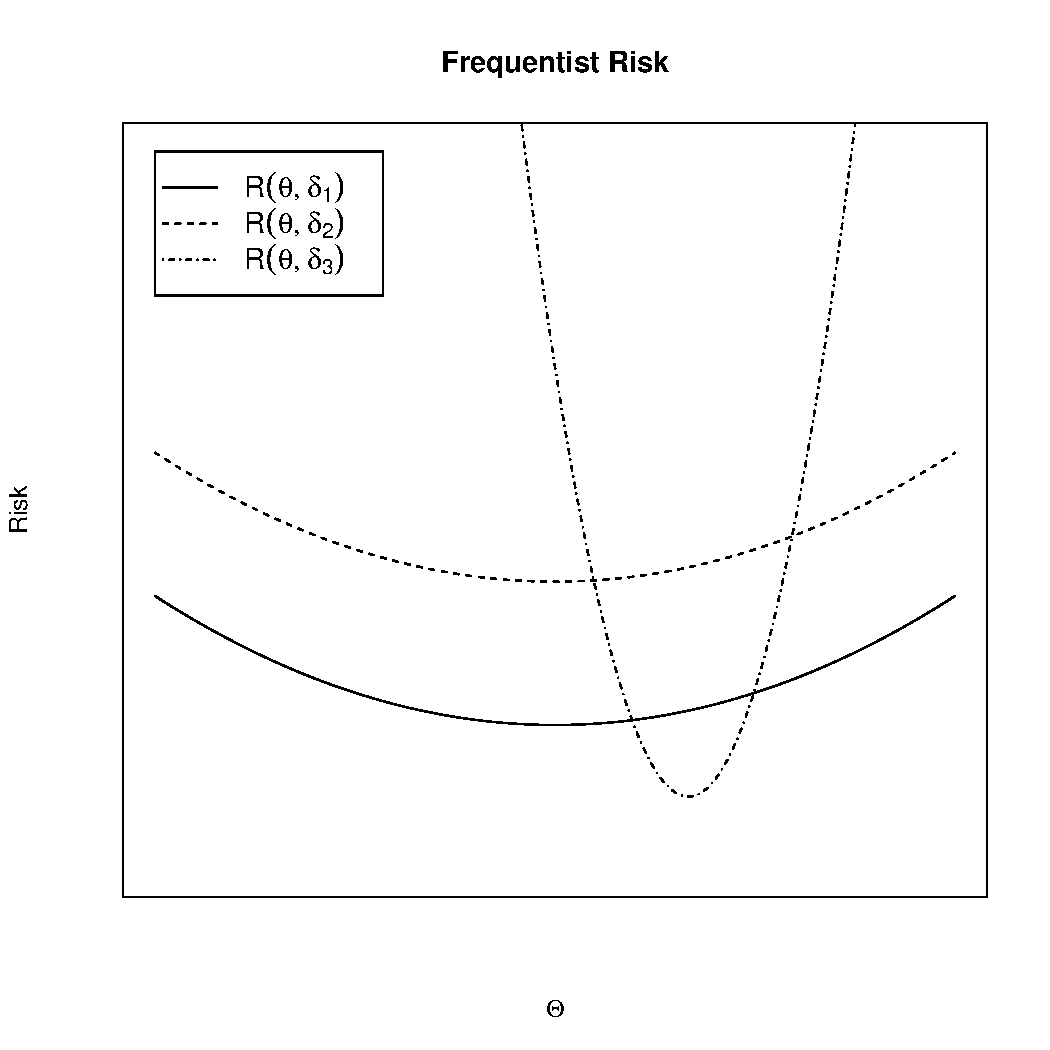
\includegraphics[width = .5\textwidth]{Lec2p1fig1.pdf}
%\caption{Shows the risk of three different decisions as a function of $\theta \in \Theta$}
%\label{default}
\end{center}
\end{figure}
Do any of the estimators dominate the other (over $\theta$)? 

\vskip 1em

Do any not?
%Often one decision does not dominate the other everywhere as is the case with decisions $\delta_1, \delta_2$. The challenge
%is in saying whether, for example, $\delta_1$ or $\delta_3$ is better. In other words, how should we aggregate over $\Theta$?
}
\frame{

Frequentists have a few answers for deciding which is better:\\
\begin{enumerate}
%\item \textbf{Admissibility}. \textbf{A decision which is inadmissible is one that is dominated everywhere.} For example, in Figure~1, $\delta_2$
%dominates $\delta_1$ for all values of $\theta.$ It would be easy to compare decisions if all but one
%were inadmissible. But usually the risk functions overlap, so this criterion fails.
\item   \textbf{Restricted classes of procedure}. 
\begin{itemize}
\item We could force $E_\theta[\hat{\theta}]=\theta$ for all $\theta$ (unbiased). 
\begin{itemize}
\item Suppose we only look at unbiased estimators.
\item Then we can often reduce the situation to only risk curves like $\delta_1$ and $\delta_2$ in Figure~1, eliminating
overlapping curves like $\delta_3$. 
\end{itemize}
\item Existence of an optimal unbiased procedure is a
nice frequentist theory, but many good procedures are biased---for example Bayesian procedures are typically
biased. 
\item Food for thought: will an unbiased estimator always exist?!?!?
%\item More surprisingly, some unbiased procedures are actually inadmissible. For example, James and 
%Stein showed that the sample mean is an inadmissible estimate of the mean of a multivariate Gaussian
%in three or more dimensions.
%\item There are also some problems were no unbiased estimator exists---for example, when $p$ is a binomial proportion and we wish to estimate $1/p$ (see Example~2.1.2 on page~83 of Lehmann and Casella).
%\item If we restrict our class of procedures to those which are equivariant, we also get nice properties. We do
%not go into detail here, but these are procedures with the same group theoretic properties as the data.
\end{itemize}
\item \textbf{Minimax}. Here, we look at $\sup_{\Theta} R(\theta,\del)$, where $$\frisk.$$ 
\begin{itemize}
\item In Figure~2, $\delta_2$ would be chosen over $\delta_1$ because its maximum worst-case risk (the grey dotted line) is
lower.
\begin{itemize}
\item Specifically, find the global max of $\delta_1$ and $\delta_2$. Now choose the minimum. This gives you the minimimax estimator which is $\delta_2$ here.
\item First, maximize over all possible $\theta \in \Theta$. Then take the minimum. 
\end{itemize}
\item sup =  supremum. See the definition given in class. 
%Think of this as finding the max\footnote{This is technically not correct but for this class it will be sufficient. In some cases, a set might not have a maximum, and then we look at the least upper bound. To learn more -- take real analysis or measure theory!}. 
\end{itemize}
\end{enumerate}
}

\frame{

\begin{figure}[htbp]
\begin{center}
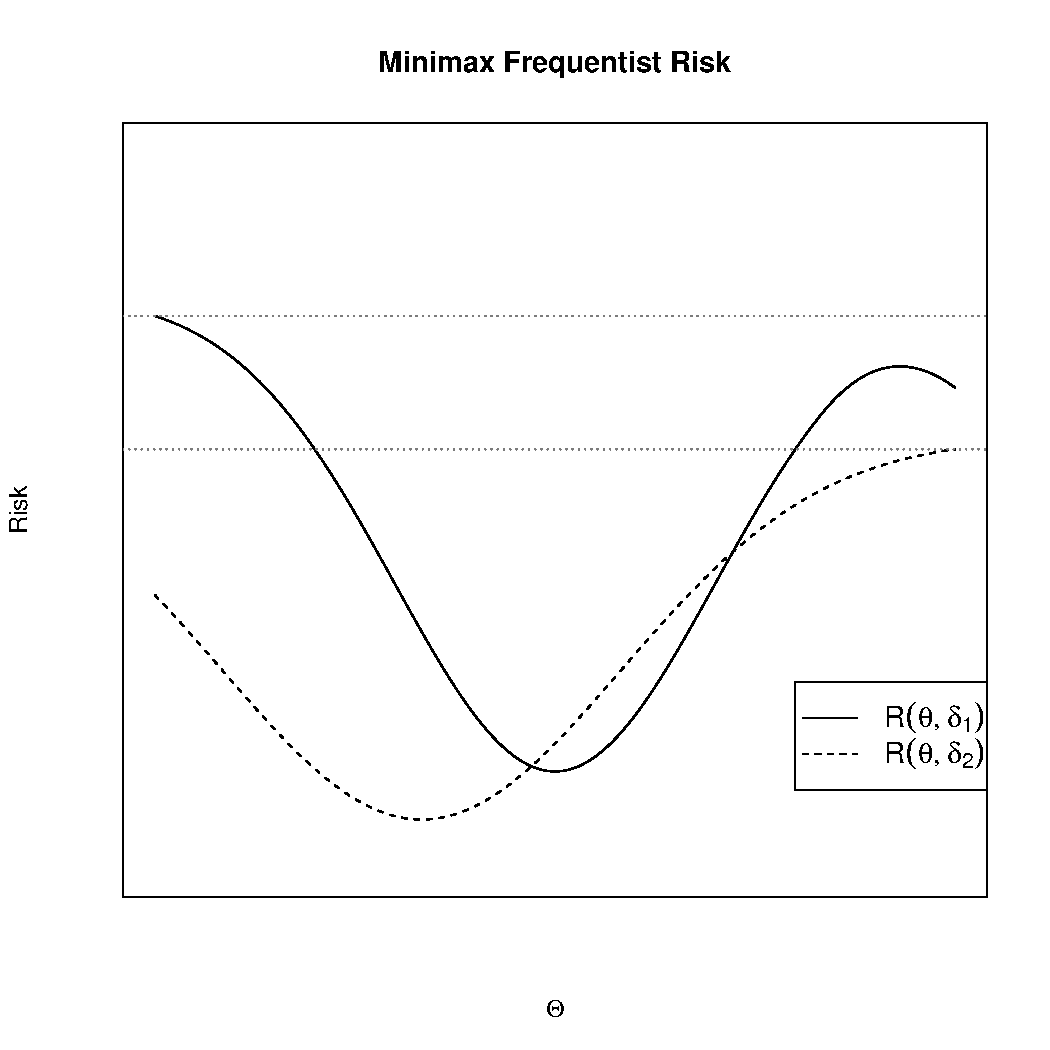
\includegraphics[width = .7\textwidth]{Lec2p2fig2.pdf}
\caption{Minimax frequentist Risk}
\label{default}
\end{center}
\end{figure}



}

\frame{
\frametitle{Bayesian Decision Theory}
Define the \blue{posterior risk} as $$\prisk.$$

\vskip 1em

The \blue{Bayes action} $\delta^*(x)$
for any fixed $x$ is the decision $\del$ that minimizes the posterior risk. 

\vskip 1em

 If the problem at hand is to estimate some unknown parameter $\theta$, then we typically call this the \blue{Bayes estimator} instead.
 
 \vskip 1em 
 
Theorem: Under squared error loss, the Bayes estimator ( $\hat{\theta}_B$) minimizes the posterior risk.  

 \vskip 1em 
 
 $\hat{\theta}_B$ happens to be the posterior mean $E(\theta \mid \bm{X})!$ 


}

\frame{


Under squared error loss, $\hat{\del}$ minimizing the posterior risk is $\hat{\theta}_B$. 
\vskip 20 em
%\begin{proof}
%Suppose that $\loss = (\tth - \del)^2.$ Now note that
%\begin{align*}
%\rho(\pi,\del) &= \int (\tth - \del)^2 \pi(\tth|x) \; d\theta \\
%&= \int \tth^2 \pi(\tth|x) \; d\theta + \del^2 \int \pi(\tth|x) \; d\theta
%-2 \del \int \tth \pi(\tth|x) \; d\theta.
%\end{align*}
%Then
%\begin{align*}
%\frac{\partial[\rho(\pi,\del)]}{\partial[\del]}  &=
%2 \del -2  \int \tth \pi(\tth|x) \; d\theta = 0 \iff \del = E[\theta|x],
%\end{align*}
%and $\partial^2[\rho(\pi,\del)]/\partial[\del]^2=2>0$, so $\del=E[\theta|x]= \hat{\theta}_B$ is the minimizer.
%\end{proof}

}

%\frame{
%In frequentist usage, the parameter $\tth$ is fixed, and thus it is the sample space over which averages are taken. Letting $R(\tth, \del)$ denote
%the frequentist risk, recall that 
%$\frisk.$ 
%\vskip 1em
%Let the loss function be squared error. In this case, the risk is
%\begin{align*}
%R(\tth, \del) &= E_{\tth}[(\tth-\del)^2]\\
%&= E_{\tth}[\left\{\tth-  E_{\tth}[\del] + E_{\tth}[\del]  - \del\right\}^2]\\
%&=\left\{\tth-  E_{\tth}[\del] \right\}^2+ E_{\tth}[\left\{\del-  E_{\tth}[\del] \right\}^2 \\
%&= \text{Bias$^2$ + Variance}
%\end{align*}
%This result allows a frequentist to analyze the variance and bias of an estimator separately, and can be used
%to motivate frequentist ideas, e.g. minimum variance unbiased estimators (MVUEs).
%
%
%
%}

%\frame{
%\frametitle{Posterior Risk}
%
%
%The posterior risk is defined as 
%$\rho(x, \pi)$ based on the data $x$ and a prior $\pi,$ where
%$$\prisk.$$
%Note that the prior enters the equation when calculating the posterior density. Using the Bayes risk, we can
%define a bit of jargon. Recall that the Bayes action $\delta^*(x)$ is the value of $\del$ that minimizes the posterior risk. We already showed that the Bayes action under squared error loss is the posterior mean. 
%
%
%
%}

\frame{
\frametitle{Bayes risk}

The Bayes risk is denoted by $r(\pi, \delta(x)).$ While the Bayes risk is a frequentist concept since it averages over $X$, the expression can also be interpreted differently. Consider
\begin{align}
r(\pi, \del) &= \int \int \loss \; f(x|\theta) \;  \; \pi(\theta)\; dx \;d\theta \\
r(\pi, \del) &= \int \int \loss \; \pi(\tth | x) \;  \; \pi(x)\; dx \;d\theta \\
r(\pi, \del) &= \int \rho(\pi,\del)  \; \pi(x)\; dx.
\end{align}
\vskip 1em
Note that the last equation is the posterior risk averaged over the marginal distribution of x.
\vskip 1em
Connection with frequentist theory includes that finding a Bayes rule against the ``worst possible
prior" gives you a minimax estimator.




}

\frame{
\frametitle{The Umbrella and the Statistician}
Suppose a statistician doesn't particularly like getting wet, so he's interested in knowing how often he should carry his umbrella given the probability that it will rain on a given day.

\begin{table}[htbp]
\begin{center}
\begin{tabular}{crcc}
&&\multicolumn{2}{c}{Statistician} \\
&& Takes Umbrella (T) & Doesn't Take (D)\\
\multirow{2}{*}{Nature} & Rain (R) & 0 & 10\\
& No Rain (N) & 1 & 0
\end{tabular}
\end{center}
\caption{Loss Function}
\label{default}
\end{table}

Consider what our loss function is in terms of the table above. 
\begin{equation*}
 L(\theta, d) =
 \begin{cases}
   0, & \text{for $L(R,T)$,} \\
   10, & \text{for $L(R,D)$,} \\
   1, & \text{for $L(N,T)$,}\\
   0, & \text{for $L(N,D)$.}
 \end{cases}
\end{equation*}
}

\frame{
\begin{itemize}
\item
Notice that in this example, there is no data $X.$ 
\item
  Thus, $R(\theta,d) = E_\theta[L(\theta,d(X))]$ is really just $E_\theta[L(\theta,d)]=L(\theta,d),$ so \textcolor{blue}{the risk and the loss} are the same. This is \emph{always} the case in no data problems.
  

\item Suppose we can predict ``Rain" with $100\%$ accuracy. 
\item Let's now find the value of $d$ that minimizes $R(\theta,d).$ 
\end{itemize}

\textcolor{blue}{Recap: we're minimizing the risk first.}
}
\frame{

Recall the loss.
\begin{equation*}
 L(\theta, d) =
 \begin{cases}
   \textcolor{blue}{0}, & \text{for $\textcolor{blue}{L(R,T)}$,} \\
   \textcolor{blue}{10}, & \text{for $\textcolor{blue}{L(R,D)}$,} \\
   1, & \text{for $L(N,T)$,}\\
   0, & \text{for $L(N,D)$.}
 \end{cases}
\end{equation*}


\emph{Solution}:
Note, I'm using R for two different things (risk and Rain)! 
\vskip 1em
Let's look at $\textcolor{blue}{\theta = (Rain)}$
\begin{equation*}
 \textcolor{red}{R}(R,d)  =
 \begin{cases}
   0, & \text{if $d=T$,} \\
   10, & \text{if $d=D$}.
 \end{cases}
\end{equation*}

\begin{itemize}
\item The $d$ that minimizes the risk above is $\textcolor{blue}{d=T},$ meaning the statistician would take his umbrella. 
\item What happens when $\theta = N$ with $100\%$ accuracy?
\end{itemize}
}

\frame{
  The cases above are unreasonable, so let's consider the situation where we know

\begin{equation*}
 \theta  =
 \begin{cases}
   R, & \text{with probability $p$,} \\
   N, & \text{with probability $1-p$.}
 \end{cases}
\end{equation*}

This is a prior $p(\theta)$ on the values of $\theta.$




}

\frame{

Now we would like to minimize the Bayes risk, $r(d) =E_X[R(\theta,d)].$ \\

Recall the loss.
\begin{equation*}
 L(\theta, d) =
 \begin{cases}
   0, & \text{for $L(R,T)$,} \\
   10, & \text{for $L(R,D)$,} \\
   1, & \text{for $L(N,T)$,}\\
   0, & \text{for $L(N,D)$.}
 \end{cases}
\end{equation*}

\emph{Solution}:
If the statistician \emph{takes the umbrella (T)}, then
$$r(d) = E_X[R(\theta,T)] = p\cdot0+(1-p)\cdot1 = 1- p.$$
If the statistician decides to \emph{does not take the umbrealla (N)} then
$$r(d) = E_X[R(\theta,D)] = p\cdot10 + (1-p)\cdot0 = 10p.$$

}

\frame{

Recall from the previous slide:
If the statistician \emph{takes the umbrella}, then
$$r(d) = E_X[R(\theta,T)] = p\cdot0+(1-p)\cdot1 = 1- p.$$
If the statistician decides to \emph{leave his umbrella} at home then
$$r(d) = E_X[R(\theta,D)] = p\cdot10 + (1-p)\cdot0 = 10p.$$

Then

\begin{itemize}
\item If $1-p < 10p,$ then the statistician should take his umbrella. 
\item On the other hand, if $1-p > 10p,$ the statistician should leave his umbrella at home. Note that we have minimized the Bayes risk. 
\end{itemize}
At home: think about what is the value of $p$ when the statistician takes and doesn't take his umbrella that results in the two situations having equal Bayes risk?
}

\frame{
\frametitle{Back to Minimaxity}

An estimator is minimax if it minimizes the maximum risk. For solving problems:
\begin{enumerate}
\item  maximize the risk over all possible parameter values, e.g. $\theta$. 
\item Then we find the estimator that minimizes this maximum risk.
\end{enumerate}

\vskip 1em

Often applying the definition can be hard. 

}

\frame{
\frametitle{More on Minimaxity}

A more useful way of showing minimaxity! 

\vskip 1em

If the Bayes estimate, $\hat{\theta}_B,$ has constant (frequentist) risk under the given prior, then $\hat{\theta}_B$ is considered to be minimax.





}

\frame{


Recall our ``umbrella example":
\begin{equation*}
 L(\theta, d) =
 \begin{cases}
   0, & \text{for $L(R,T)$,} \\
   10, & \text{for $L(R,D)$,} \\
   1, & \text{for $L(N,T)$,}\\
   0, & \text{for $L(N,D)$.}
 \end{cases}
\end{equation*}
\begin{itemize}
\item  This is a no data problem, so $R(\theta,d) = L(\theta,d).$ 
\item Then to find the minimax estimator $d$, we first maximize over all possible values of $\theta$ for each estimator $d$, i.e., we maximize over rain and not rain. 
\item The maximum risks for $D$ and $T$ are $R(R,D) = 10$ and $R(N,T) =1.$ Then minimizing the risk functions over the estimators, we find $R(N,T) = 1.$ 
\item So, the minimax estimator is $d=T$, or rather for the statistician to \emph{always} carry his umbrella.
\item How would this change with a prior on $\theta$? Think about this at home. 
\end{itemize}

}












\end{document}